\documentclass[conference]{IEEEtran}

\usepackage[utf8]{inputenc}
\usepackage[T1]{fontenc}
\usepackage[brazil]{babel}
\usepackage{cite}
\usepackage{amsmath,amssymb,amsfonts}
\usepackage{graphicx}
\usepackage{textcomp}
\usepackage{xcolor}
\usepackage{booktabs}
\usepackage{multirow}
\usepackage{array}
\usepackage{tabularx}
\usepackage{newunicodechar}
\usepackage{tikz}
\usetikzlibrary{positioning,arrows.meta,calc}
\usepackage[hidelinks]{hyperref}

\newunicodechar{−}{\ensuremath{-}}
\newunicodechar{≈}{\ensuremath{\approx}}
\newunicodechar{≤}{\ensuremath{\leq}}
\newunicodechar{≥}{\ensuremath{\geq}}
\newunicodechar{→}{\ensuremath{\rightarrow}}
\newunicodechar{×}{\ensuremath{\times}}
\newunicodechar{·}{\ensuremath{\cdot}}

% nomes das métricas: nomes próprios, em itálico, como nos artigos de origem
\newcommand{\FC}{\textit{Faithfulness Correlation}}
\newcommand{\FE}{\textit{Faithfulness Estimate}}
\newcommand{\MS}{\textit{Max-Sensitivity}}
\newcommand{\AS}{\textit{Avg-Sensitivity}}
\newcommand{\CX}{\textit{Complexity}}
\newcommand{\CS}{\textit{Consistency}}
\newcommand{\RL}{\textit{Random Logit}}
\newcommand{\EM}{eMPRT}

\tikzset{
  caixa/.style={draw=black!70, rounded corners=2pt, align=center, font=\footnotesize, inner sep=3pt, fill=white},
  dado/.style={caixa, fill=blue!6},
  proc/.style={caixa, fill=orange!8},
  saida/.style={caixa, fill=green!7},
  seta/.style={-{Stealth[length=2mm]}, thick, black!70},
  nota/.style={font=\scriptsize, text=black!65, align=center},
}

\renewcommand{\IEEEkeywordsname}{Palavras-chave}

\begin{document}

\title{Avaliação das Explicações SHAP em Redes Neurais Profundas para Classificação de Arritmias Cardíacas em ECG}

\author{
\IEEEauthorblockN{Arthur Santos de Oliveira}
\IEEEauthorblockA{
\textit{Instituto de Ciência e Tecnologia}\\
\textit{Universidade Federal de São Paulo}\\
São José dos Campos, Brasil\\
oliveira.arthur@unifesp.br}
\and
\IEEEauthorblockN{Luis Augusto Martins Pereira}
\IEEEauthorblockA{
\textit{Instituto de Ciência e Tecnologia}\\
\textit{Universidade Federal de São Paulo}\\
São José dos Campos, Brasil\\
luis.pereira@unifesp.br}
}

\maketitle

\begin{abstract}
Redes neurais profundas classificam arritmias no eletrocardiograma (ECG) com bom desempenho, mas o desempenho varia entre as classes diagnósticas, e não se sabe se a qualidade das explicações acompanha essa variação. Este estudo investigou se a qualidade das explicações GradientSHAP de uma ResNet34 unidimensional acompanha o F1 por classe. O modelo foi treinado na base CPSC2018 (nove classes, ECG de 12 derivações) e obteve F1-macro de 0,819 no teste. Foram gerados 622 mapas de atribuição para as predições corretas, e cada mapa foi resumido em 36 regiões fisiológicas (12 derivações × pré-QRS, QRS e ST-T) ancoradas nos picos R. Sete métricas quantitativas foram reimplementadas sobre essas regiões e lidas em relação à variação própria do método entre sementes aleatórias. As métricas que envolvem a decisão do modelo entre classes (\CS\ e \RL) acompanharam o F1 nas pontas: as classes de maior F1 tiveram explicações mais consistentes e mais específicas. As de fidelidade e de robustez não acompanharam o F1 e seguiram o tipo de evidência da classe, com as classes reconhecidas pela forma do QRS no alto e as de ritmo e de segmento ST embaixo. A relação entre qualidade da explicação e desempenho depende, portanto, da propriedade medida, e diferenças de fidelidade entre classes não devem ser lidas como diferenças de confiabilidade sem considerar a amplitude e a duração da evidência de cada classe.
\end{abstract}

\begin{IEEEkeywords}
eletrocardiograma, arritmias, inteligência artificial explicável, SHAP, avaliação de explicações
\end{IEEEkeywords}

\section{Introdução}\label{sec:introducao}

As doenças cardiovasculares são a principal causa de morte, e o eletrocardiograma (ECG) é um meio simples, confiável e não invasivo de acompanhar a atividade do coração e de diagnosticar arritmias~\cite{zhang2021}. O ECG padrão tem 12 derivações, registradas ao mesmo tempo por eletrodos na superfície do corpo~\cite{zhang2021}. Em cada derivação, cada batimento aparece como uma sequência de ondas e segmentos, como a onda P, o complexo QRS, o segmento ST e a onda T, cujas amplitudes diferem muito entre si, com o pico R do QRS dominando o traçado~\cite{gumpfer2026}. Os diagnósticos se apoiam em partes diferentes dessa sequência: alguns na forma do QRS, de grande amplitude, como os bloqueios de ramo; outros em segmentos de baixa amplitude, próximos da linha de base, como na isquemia, que altera o segmento ST~\cite{gumpfer2026}. Como interpretar o ECG é difícil mesmo para cardiologistas experientes e o número de exames é grande, o diagnóstico automático tornou-se um tema de pesquisa ativo~\cite{zhang2021}.

Redes neurais profundas aprendem esse diagnóstico diretamente do sinal. Na base CPSC2018, com nove classes diagnósticas, uma rede residual unidimensional de 34 camadas obteve F1 médio de 0,813~\cite{zhang2021}. O desempenho, porém, não foi uniforme entre as classes: o F1 passou de 0,9 na fibrilação atrial e no bloqueio de ramo direito e foi de 0,535 na elevação do segmento ST, diferença que os autores atribuíram em parte à discordância entre médicos no diagnóstico dessa classe~\cite{zhang2021}.

Esses modelos são, em geral, considerados caixas-pretas, porque as suas decisões não podem ser rastreadas por uma pessoa, o que pesa sobretudo na prática clínica~\cite{zhang2021}. Os métodos de explicação \emph{post hoc} procuram contornar esse problema sem mudar o modelo já treinado~\cite{turbe2023}: para uma predição, atribuem a cada ponto da entrada um valor que indica quanto ele contribuiu para a saída, formando um mapa de atribuição sobre o traçado. O SHAP é um desses métodos. Ele distribui entre os atributos da entrada a diferença entre a saída do modelo e um valor de base, a saída esperada quando nenhum atributo é conhecido, de modo que a soma das atribuições reproduz essa diferença~\cite{lundberg2017}. Em redes profundas, essa distribuição é aproximada a partir dos gradientes do modelo; o GradientSHAP, por exemplo, multiplica gradientes pela diferença entre a entrada e exemplos de referência~\cite{kokhlikyan2020}. O SHAP já foi usado para explicar as predições da rede residual no CPSC2018, por paciente e por derivação~\cite{zhang2021}.

Um mapa de atribuição, contudo, não garante que descreve o modelo. Em geral, não há uma explicação correta conhecida com a qual compará-lo, e a inspeção visual é um guia fraco: mapas que não dependem do modelo nem dos dados podem ser visualmente parecidos com mapas de saliência~\cite{adebayo2018}. Por isso, foram propostas métricas quantitativas, organizadas em categorias que medem propriedades diferentes das explicações~\cite{hedstrom2023quantus}. As de \emph{fidelidade} verificam se os atributos indicados como importantes são os que mais alteram a saída quando retirados~\cite{bhatt2020}; as de \emph{robustez}, se a explicação muda pouco quando a entrada muda pouco~\cite{yeh2019}; as de \emph{complexidade}, se a importância se concentra em poucos atributos~\cite{bhatt2020}; e as de \emph{randomização}, se a explicação depende do que o modelo aprendeu e da classe explicada~\cite{adebayo2018,sixt2020}.

Em ECG e em séries temporais, essas avaliações mostraram que a qualidade das explicações não é uniforme. A \FC~\cite{bhatt2020}, uma métrica de fidelidade, foi usada para comparar onze métodos de atribuição em quatro bases de ECG~\cite{suh2024}. Quando confrontadas com regiões definidas por diretrizes clínicas, as explicações de métodos que multiplicam o gradiente pela entrada ou subtraem uma referência, entre eles o GradientSHAP, seguiram a amplitude do sinal e deixaram de cobrir regiões de baixa amplitude importantes para o diagnóstico~\cite{gumpfer2026}. Em séries temporais, a eficácia das métricas de perturbação variou muito entre as classes~\cite{baer2025a}, e diferenças simples de amplitude ou de duração do padrão entre as classes bastaram para produzir esse efeito~\cite{baer2025b}.

Esses trabalhos, porém, não relacionam a qualidade das explicações com o desempenho do modelo em cada classe. As comparações de métodos costumam usar classificadores de desempenho alto: o XTSC-Bench avalia apenas modelos com acurácia acima de 90\%~\cite{hollig2023}, e a comparação de Ismail et al.\ relata resultados de modelos com acurácia acima de 95\%~\cite{ismail2020}. Em ECG, um estudo com nove classes usou modelos com AUPRC média acima de 0,85 em oito delas~\cite{arends2026}. Assim, quando o desempenho do modelo é desigual entre as classes, como no CPSC2018, não se sabe se as classes em que o modelo mais acerta são também as de explicações de melhor qualidade.

Essa relação importa para o uso das explicações como apoio ao diagnóstico. Se a qualidade das explicações acompanhar o desempenho, as classes em que o modelo mais erra serão também aquelas em que as explicações menos merecem confiança, e o desempenho poderá servir de indicador da confiabilidade da explicação; se não acompanhar, a qualidade da explicação precisará ser avaliada à parte, classe a classe. A pergunta que orientou este estudo foi, portanto: \emph{a qualidade das explicações GradientSHAP de uma rede neural profunda para classificação de arritmias em ECG acompanha o desempenho (F1) do modelo em cada classe?}

Este estudo comparou, classe a classe, sete métricas de qualidade das explicações com o F1 de uma rede residual treinada no CPSC2018 e mostrou que a resposta depende da propriedade medida. As métricas que envolvem a decisão do modelo entre classes acompanharam o F1 nas classes de melhor e de pior desempenho, enquanto as de fidelidade e de robustez acompanharam o tipo de evidência de cada classe, e não o seu desempenho.

\section{Metodologia}\label{sec:metodologia}

Para responder à pergunta do estudo, eram necessárias duas medidas para cada classe diagnóstica: o desempenho do modelo e a qualidade das explicações das suas predições. O estudo foi, por isso, experimental e descritivo, com a classe como unidade de comparação (Fig.~\ref{fig:pipeline}). Um classificador multirrótulo foi treinado, e o seu desempenho em cada classe foi medido pelo F1 no conjunto de teste. As predições corretas desse conjunto foram explicadas pelo GradientSHAP, cada explicação foi resumida em regiões do batimento, e a qualidade das explicações foi medida por sete métricas de quatro categorias, para que a pergunta fosse respondida para várias propriedades, e não para uma só. Por fim, a ordem das classes em cada métrica foi comparada com a ordem pelo F1. Todo o código e os resultados estão em um repositório público\footnote{\url{https://github.com/Arthur-so/shap-ecg-arrhythmia}}.

\begin{figure*}[!t]\centering
\begin{tikzpicture}[node distance=5mm and 7mm]
\node[dado] (d) {CPSC2018\\6\,877 ECGs\\12 derivações};
\node[proc, right=of d] (p) {Pré-processamento\\(Seção~\ref{sec:dados})};
\node[proc, right=of p] (m) {Treino da\\ResNet34-1D\\(Seção~\ref{sec:modelo})};
\node[saida, right=of m] (f) {F1 por classe\\no teste};
\node[proc, below=8mm of m] (g) {GradientSHAP\\622 mapas\\(Seção~\ref{sec:gshap})};
\node[proc, left=of g] (r) {36 regiões\\do batimento\\(Seção~\ref{sec:regioes})};
\node[proc, left=of r] (mt) {7 métricas + piso\\(Seções~\ref{sec:piso}\\e~\ref{sec:metricas})};
\node[saida, right=of g] (c) {Comparação\\descritiva\\(Seção~\ref{sec:analise})};
\draw[seta] (d) -- (p); \draw[seta] (p) -- (m); \draw[seta] (m) -- (f);
\draw[seta] (m) -- (g); \draw[seta] (g) -- (r); \draw[seta] (r) -- (mt);
\draw[seta] (f) -- (c);
\draw[seta] (mt.south) -- ++(0,-4mm) -| (c.south);
\end{tikzpicture}

\caption{Etapas do estudo. O desempenho do modelo (F1 por classe, em cima) e a qualidade das explicações (métricas por classe, embaixo) foram obtidos para as mesmas classes e comparados ao final.}\label{fig:pipeline}
\end{figure*}

\subsection{Base de dados e pré-processamento}\label{sec:dados}
Foi usada a base do \textit{China Physiological Signal Challenge} 2018 (CPSC2018)~\cite{liu2018}, na distribuição do desafio PhysioNet/CinC 2020~\cite{perezalday2020}: 6\,877 ECGs de 12 derivações amostrados a 500~Hz, com duração de 6 a 60~s~\cite{zhang2021}. Os rótulos foram lidos dos códigos SNOMED CT dos cabeçalhos e mapeados para nove classes: ritmo sinusal normal (SNR), fibrilação atrial (AF), bloqueio atrioventricular de 1.º grau (IAVB), bloqueio de ramo esquerdo (BRE), bloqueio de ramo direito (BRD), contração atrial prematura (CAP), contração ventricular prematura (CVP), depressão do segmento ST (STD) e elevação do segmento ST (STE). Como 476 registros (6,9\%) tinham mais de um diagnóstico, o problema foi tratado como multirrótulo. A Tabela~\ref{tab:classes} mostra o número de registros por classe.

\begin{table}[!t]\centering
\caption{Registros por classe em cada partição. Um registro pode ter mais de um rótulo.}\label{tab:classes}
\setlength{\tabcolsep}{4pt}
\begin{tabular}{lrrrr}
\toprule
\textbf{Classe} & \textbf{Treino} & \textbf{Validação} & \textbf{Teste} & \textbf{Total} \\
\midrule
SNR  & 642 & 184 & 92 & 918 \\
AF   & 858 & 242 & 121 & 1\,221 \\
IAVB & 503 & 144 & 75 & 722 \\
BRE  & 165 & 47 & 24 & 236 \\
BRD  & 1\,304 & 371 & 182 & 1\,857 \\
CAP  & 431 & 122 & 63 & 616 \\
CVP  & 491 & 140 & 69 & 700 \\
STD  & 609 & 172 & 88 & 869 \\
STE  & 154 & 44 & 22 & 220 \\
\midrule
Registros & 4\,812 & 1\,378 & 687 & 6\,877 \\
\bottomrule
\end{tabular}
\end{table}

Como a rede exige entradas de tamanho fixo, cada registro foi truncado ou completado com zeros até 15\,000 amostras (30~s), o mesmo comprimento usado por Zhang et al.~\cite{zhang2021}. Diferentemente da referência, que mantém os últimos 30~s dos registros longos e não normaliza o sinal~\cite{zhang2021}, foram mantidos os primeiros 30~s, e cada derivação foi normalizada por \textit{z-score}; por isso, as amplitudes estão em unidades de desvio padrão. Os registros foram divididos em treino, validação e teste (70\%, 20\% e 10\%), de forma estratificada por classe e com semente fixa. O comprimento real de cada registro foi guardado para excluir o preenchimento de todas as análises por região, já que a duração mediana dos registros era de 12~s.

\subsection{Modelo e treino}\label{sec:modelo}
Foi usada a ResNet34 unidimensional de Zhang et al.~\cite{zhang2021}, por ser a arquitetura de referência na mesma base, adaptada das redes residuais de He et al.~\cite{he2016}, em que cada bloco aprende um resíduo em relação à sua entrada, somada à saída por uma conexão de atalho (Fig.~\ref{fig:resnet}). As 12 derivações entram na rede como canais; dezesseis blocos residuais em quatro estágios reduzem o sinal a 512 canais × 469 instantes; a média e o máximo ao longo do tempo formam um vetor de 1\,024 valores; e uma camada linear produz um logit $z_c$ por classe. A probabilidade de cada classe foi obtida por uma sigmoide independente, $p_c = 1/(1+e^{-z_c})$, porque um ECG pode ter mais de um diagnóstico, e a classe foi considerada predita quando $p_c$ atingiu o limiar $t_c$ da classe.

\begin{figure*}[!t]\centering
\begin{tikzpicture}[node distance=3mm and 3.2mm, every node/.style={font=\scriptsize}]
\node[dado, minimum height=11mm] (in) {ECG\\12 × 15\,000};
\node[proc, right=of in, minimum height=11mm] (st) {Conv 15, /2\\BN, ReLU\\MaxPool /2};
\node[proc, right=of st, minimum height=11mm, fill=orange!15] (s1) {Estágio 1\\3 blocos};
\node[proc, right=of s1, minimum height=11mm, fill=orange!22] (s2) {Estágio 2\\4 blocos, /2};
\node[proc, right=of s2, minimum height=11mm, fill=orange!30] (s3) {Estágio 3\\6 blocos, /2};
\node[proc, right=of s3, minimum height=11mm, fill=orange!38] (s4) {Estágio 4\\3 blocos, /2};
\foreach \n/\t in {in/{12 × 15\,000}, st/{64 × 3\,750}, s1/{64 × 3\,750}, s2/{128 × 1\,875}, s3/{256 × 938}, s4/{512 × 469}}
  \node[nota, below=0.5mm of \n] {\t};
\node[proc, below=11mm of s4, minimum height=11mm] (pool) {Média e máximo\\no tempo};
\node[proc, below=11mm of s3, minimum height=11mm] (fc) {Linear\\1\,024 → 9};
\node[proc, below=11mm of s2, minimum height=11mm] (sig) {Sigmoide\\por classe};
\node[proc, below=11mm of s1, minimum height=11mm] (lim) {$p_c \ge t_c$\,?};
\node[saida, below=11mm of st, minimum height=11mm] (out) {Classes\\preditas};
\node[nota, below=0.5mm of pool] {1\,024};
\node[nota, below=0.5mm of fc] {9 logits\\$z_c$};
\node[nota, below=0.5mm of sig] {9 probabilidades\\$p_c$};
\node[nota, below=0.5mm of lim] {limiar $t_c$\\por classe};
\draw[seta] (in)--(st); \draw[seta] (st)--(s1); \draw[seta] (s1)--(s2); \draw[seta] (s2)--(s3); \draw[seta] (s3)--(s4);
\draw[seta] (s4)--(pool); \draw[seta] (pool)--(fc); \draw[seta] (fc)--(sig); \draw[seta] (sig)--(lim); \draw[seta] (lim)--(out);
% bloco residual
\begin{scope}[shift={(1.2,-4.75)}, node distance=2.6mm]
\node[font=\scriptsize\bfseries, anchor=east] (tit) at (-0.85,0) {Bloco residual:};
\node[caixa, font=\scriptsize] (x) {entrada};
\node[caixa, right=of x, font=\scriptsize] (c1) {Conv 7};
\node[caixa, right=of c1, font=\scriptsize] (b1) {BN, ReLU};
\node[caixa, right=of b1, font=\scriptsize] (dp) {\textit{Dropout} 0,2};
\node[caixa, right=of dp, font=\scriptsize] (c2) {Conv 7};
\node[caixa, right=of c2, font=\scriptsize] (b2) {BN};
\node[circle, draw, right=of b2, inner sep=1pt, font=\scriptsize] (sum) {$+$};
\node[caixa, right=of sum, font=\scriptsize] (rl) {ReLU};
\draw[seta] (x)--(c1); \draw[seta] (c1)--(b1); \draw[seta] (b1)--(dp); \draw[seta] (dp)--(c2); \draw[seta] (c2)--(b2); \draw[seta] (b2)--(sum); \draw[seta] (sum)--(rl);
\draw[seta] (x.south) -- ++(0,-4mm) -| (sum.south);
\node[nota, below=4.5mm of dp] {atalho: a entrada é somada à saída (com Conv 1 × 1, /2, quando o comprimento muda)};
\end{scope}
\end{tikzpicture}

\caption{Arquitetura da ResNet34-1D: o ECG atravessa quatro estágios de blocos residuais, é resumido no tempo e produz um logit e uma probabilidade por classe. Abaixo de cada etapa, a dimensão da saída (canais × instantes); embaixo, um bloco residual, em que a entrada é somada à saída. Elaborada com base em~\cite{zhang2021}.}\label{fig:resnet}
\end{figure*}

O treino usou entropia cruzada binária sem ponderação, otimizador Adam com taxa de aprendizado $10^{-4}$, lotes de 32 ECGs, \textit{dropout} de 0,2 nos blocos e aumento de dados por escala e deslocamento da linha de base de cada derivação, como na referência~\cite{zhang2021}. O treino foi limitado a 60 épocas, com parada antecipada após 10 épocas sem melhora do F1-macro na validação, e foi mantido o modelo da melhor época; a referência usa no máximo 30 épocas~\cite{zhang2021}. Para verificar se o desbalanceamento entre as classes exigia uma perda ponderada, foi treinado também um modelo com a entropia cruzada ponderada pela frequência de cada classe, nas mesmas condições.

Como o limiar que maximiza o F1 em geral não é 0,5 e depende da classe~\cite{lipton2014}, o limiar de cada classe foi escolhido na validação, testando valores de 0,00 a 1,00 em passos de 0,01 e escolhendo o de maior F1, e depois aplicado sem mudança ao teste, como em~\cite{zhang2021}. O desempenho foi medido pelo F1 de cada classe no teste, e o F1-macro, a média das nove classes, foi usado como resumo.

\subsection{Explicações GradientSHAP}\label{sec:gshap}
Para cada ECG $x$ e classe $c$, o GradientSHAP, na implementação do Captum~\cite{kokhlikyan2020}, produziu um mapa $\phi$ com a mesma dimensão do ECG (12 × 15\,000), que atribui a cada ponto uma parcela do logit $z_c$. O método aproxima os valores SHAP~\cite{lundberg2017} por gradientes calculados ao longo do caminho entre referências e a entrada, como nos gradientes integrados~\cite{sundararajan2017}. Em cada um de $M = 200$ sorteios, foram sorteados uma referência $r_m$ e um ruído gaussiano somado ao ECG, $\tilde{x}_m = x + \varepsilon_m$; foi sorteado um ponto $x'_m = r_m + \alpha_m(\tilde{x}_m - r_m)$ do caminho entre os dois, com $\alpha_m \in [0,1]$; e o gradiente nesse ponto foi multiplicado pela diferença entre o ECG e a referência (Fig.~\ref{fig:gshap}). O mapa é a média dos sorteios:
\begin{equation}
\phi(x) = \frac{1}{M}\sum_{m=1}^{M} \nabla z_c(x'_m) \odot (\tilde{x}_m - r_m).
\label{eq:gshap}
\end{equation}

\begin{figure*}[!t]\centering
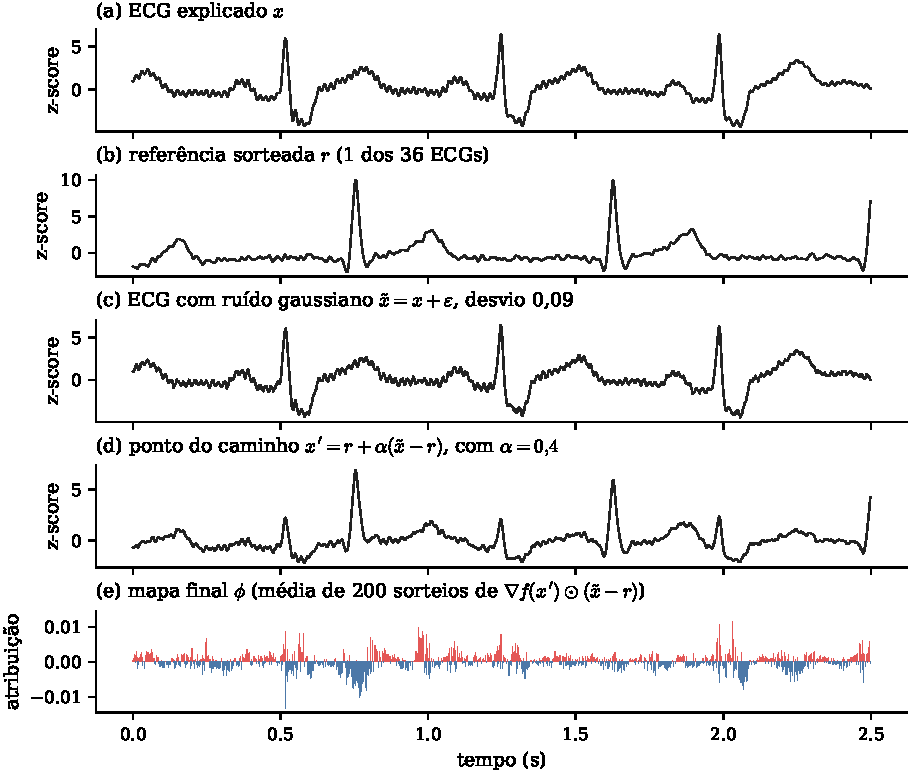
\includegraphics[width=0.6\textwidth]{figs/gshap.pdf}
\caption{Construção de um mapa GradientSHAP com sinais reais (derivação II de um ECG de BRD). Os painéis (a) a (d) mostram um sorteio: (a) ECG; (b) uma das 36 referências; (c) ECG com ruído; (d) ponto do caminho em que o gradiente é calculado. O painel (e) mostra o mapa final, média de 200 sorteios, com a atribuição positiva em vermelho e a negativa em azul; os maiores valores ficam nos complexos QRS.}\label{fig:gshap}
\end{figure*}

As referências foram 36 ECGs do treino com um único rótulo, quatro de cada classe, sorteados com semente fixa. Usar uma distribuição de ECGs reais como referência segue Turbé et al.~\cite{turbe2023}, que usaram 50 ECGs na mesma base; o balanceamento evita que a referência represente sobretudo as classes mais frequentes. O ruído suaviza oscilações locais do gradiente, como no SmoothGrad~\cite{smilkov2017}; o desvio usado, 0,09, é o do exemplo de uso do Captum e não foi ajustado. O número de sorteios foi aumentado de 50 para 200 depois que a variação entre mapas do mesmo ECG com sementes diferentes (Seção~\ref{sec:piso}) se mostrou alta com 50; com 200, essa variação caiu à metade. Foram explicadas apenas as predições corretas do teste: para cada registro, um mapa para cada classe presente e predita, num total de 622 mapas.

\subsection{Regiões do batimento}\label{sec:regioes}
Cada mapa tinha 180\,000 valores. As métricas, porém, foram calculadas sobre 36 regiões, e não sobre pontos, por três motivos. Primeiro, retirar pontos isolados quase não altera a saída do modelo e incluía o preenchimento, que ocupa a maior parte do mapa na maioria dos ECGs; perturbar trechos contíguos introduz menos ruído de alta frequência no sinal~\cite{cui2023}; agrupar pontos consecutivos melhorou as métricas de perturbação em séries temporais multivariadas~\cite{serramazza2024}; e perturbações mínimas de pontos podem mudar bruscamente a predição por deslocamento de distribuição, o que levou à recomendação de perturbar regiões de tamanho fixo~\cite{simic2025}. Segundo, regiões como o QRS de V1 têm significado clínico. Terceiro, somar pontos reduz o ruído do mapa: numa verificação preliminar, a distância normalizada entre dois mapas do mesmo ECG com sementes diferentes (Seção~\ref{sec:piso}) foi de 0,53 nos 180\,000 pontos e de 0,18 nas 36 regiões. A agregação entre batimentos também reduz o ruído dos métodos de gradiente em ECG~\cite{wagner2024}.

Os picos R foram detectados na derivação II com o NeuroKit2~\cite{makowski2021}, e cada batimento completo, entre dois picos R, foi dividido em três segmentos (Fig.~\ref{fig:regioes}): QRS, de $R - 80$~ms a $R + 100$~ms; ST-T, de $R + 100$~ms a $R + 0{,}45 \cdot RR$; e pré-QRS, de $R + 0{,}45 \cdot RR$ até 80~ms antes do pico R seguinte, que contém a onda P e o intervalo PR. Janelas fixas em torno do pico R também foram usadas por Wagner et al.~\cite{wagner2024} (300~ms antes e 500~ms depois do pico R) e por Turbé et al.~\cite{turbe2023} (0,35~s antes e 0,55~s depois). A delineação de cada onda pelo NeuroKit2 foi testada e descartada, porque indicava ondas P em ECGs de fibrilação atrial e não reconhecia o QRS alargado dos bloqueios de ramo.

\begin{figure*}[!t]\centering
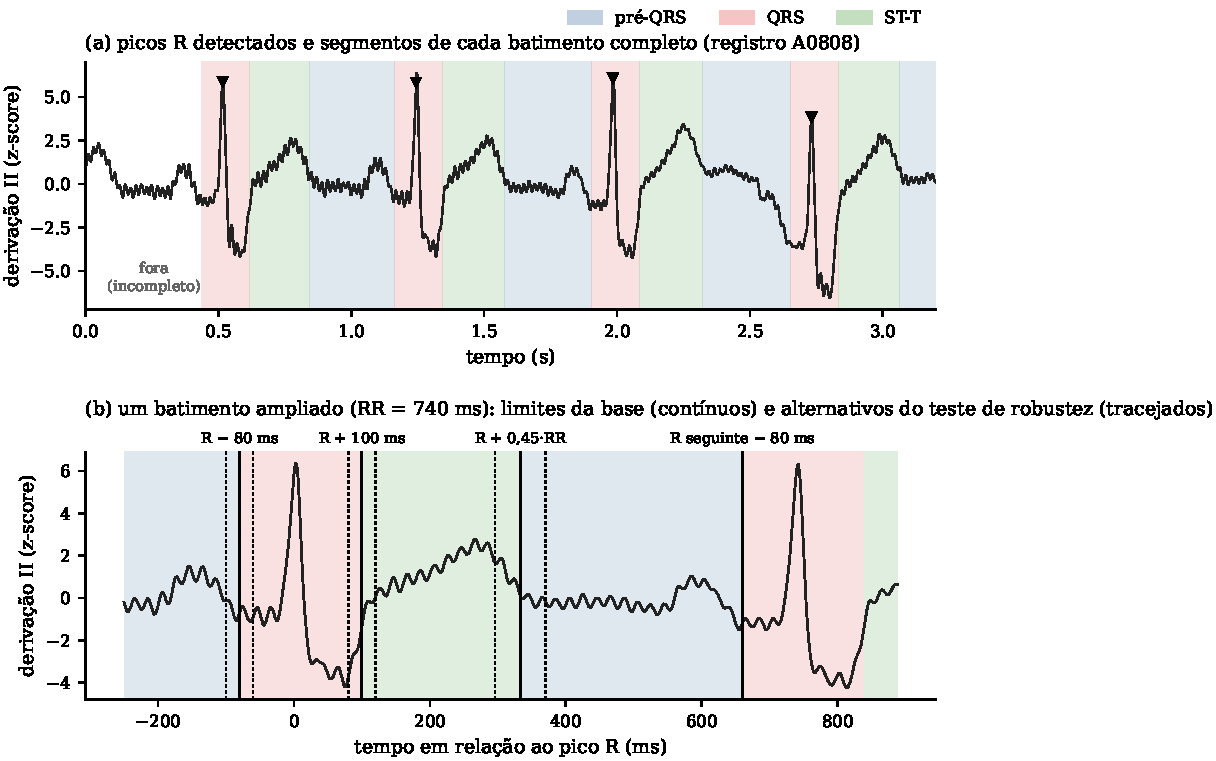
\includegraphics[width=0.72\textwidth]{figs/regioes.pdf}
\caption{Segmentos do batimento definidos a partir dos picos R, num ECG de BRD (derivação II). (a) Picos R detectados e os três segmentos de cada batimento completo; o trecho antes do primeiro pico R fica de fora. (b) Um batimento ampliado, com os limites usados (linhas contínuas) e os limites alternativos do teste de robustez (tracejadas).}\label{fig:regioes}
\end{figure*}

A janela de 180~ms cobre o QRS normal e o QRS alargado dos bloqueios de ramo, definidos por duração de 120~ms ou mais~\cite{hicks2021}; ela é maior depois do pico R porque, nesses bloqueios, o atraso de condução alonga sobretudo a parte final do QRS. O fim do ST-T foi definido como fração do intervalo RR, porque o QT encurta quando a frequência aumenta. Pela fórmula de Bazett, $QT_c = QT/\sqrt{RR}$, a correção mais usada na clínica~\cite{vandenberk2016}, um $QT_c$ de 0,44~s ocupa 0,44 do RR a 60~bpm e 0,50 a 77~bpm, a frequência mediana dos ECGs explicados. Como essa fórmula sobrecorrige o QT em frequências altas~\cite{vandenberk2016}, o fim da onda T pode cair no pré-QRS nos ECGs mais rápidos (17\% dos explicados estavam acima de 100~bpm). Como esses limites são aproximações, foram variados num teste de robustez: janela do QRS de 140, 180 ou 220~ms e fim do ST-T em 0,40, 0,45 ou 0,50 do RR, em 9 combinações, recalculando as métricas que dependem só do mapa e das regiões (\CS\ e \CX). As demais exigiriam passar pelo modelo os ECGs modificados em cada combinação e não foram recalculadas.

A importância de uma região foi definida como a soma do mapa nos pontos daquele segmento, em todos os batimentos completos, numa derivação (Fig.~\ref{fig:agregacao}):
\begin{equation}
A_{d,s} = \sum_{b} \sum_{t \in s(b)} \phi_{d,t},
\label{eq:regiao}
\end{equation}
em que $d$ é a derivação, $s$ o segmento e $b$ percorre os batimentos completos. Cada mapa foi, assim, resumido num vetor de 36 valores. A soma, e não a média usada por Wagner et al.~\cite{wagner2024}, foi escolhida porque é a quantidade que as métricas de retirada comparam com a queda da saída, e porque Zhang et al.\ também resumem os valores SHAP pela soma ao longo do tempo~\cite{zhang2021}.

\begin{figure*}[!t]\centering
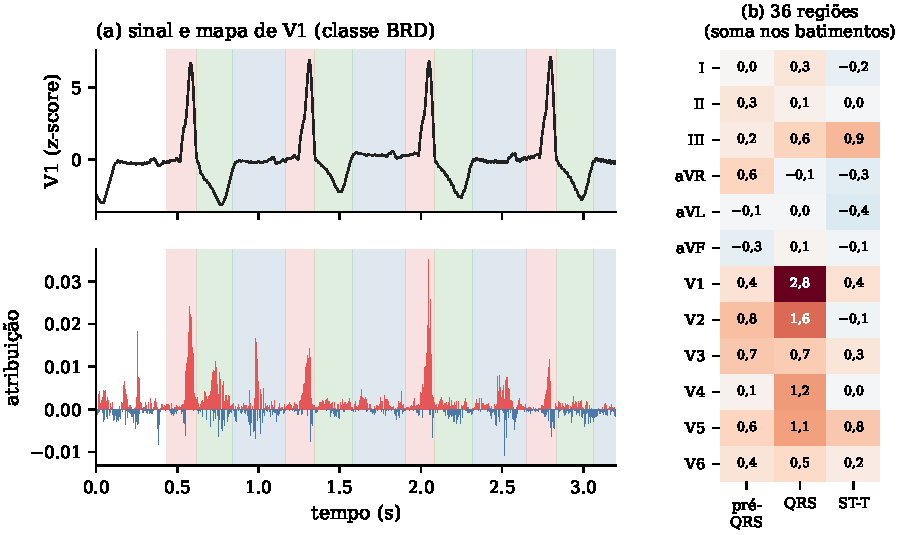
\includegraphics[width=0.74\textwidth]{figs/agregacao.pdf}
\caption{Resumo de um mapa nas 36 regiões (ECG de BRD): o mapa, que oscila ponto a ponto, concentra-se nos QRS, e no vetor das regiões o maior valor é o QRS de V1. (a) Sinal e mapa da derivação V1 nos primeiros 3,2~s, com os segmentos sombreados. (b) Vetor das 36 regiões do ECG inteiro; cada valor é a soma do mapa naquela derivação e segmento, em todos os batimentos completos.}\label{fig:agregacao}
\end{figure*}

\subsection{Variação própria do método: o piso}\label{sec:piso}
Como o GradientSHAP sorteia referências, ruído e pontos do caminho, dois mapas do mesmo ECG com sementes diferentes não são iguais. O \emph{piso} de um mapa foi definido como a distância euclidiana entre esses dois mapas, cada um resumido nas 36 regiões e normalizado para norma 1; ele vai de 0 (mapas iguais) a 2 (opostos). As três métricas que comparam mapas (\MS\ e \AS, \RL\ e \EM) foram calculadas com a mesma semente do mapa original, de modo que só muda o ECG, a classe ou o modelo, e a distância obtida foi lida em relação ao piso (Fig.~\ref{fig:piso}). Sem normalização, métodos cujos escores têm escala menor podem parecer menos sensíveis só por causa da escala~\cite{fouladgar2022}. 

\begin{figure*}[!t]\centering
\begin{tikzpicture}[node distance=4mm and 5mm, every node/.style={font=\scriptsize}]
\node[dado] (x) {ECG $x$,\\classe $c$};
\node[proc, right=10mm of x, yshift=6mm] (g1) {GradientSHAP\\semente $s_1$};
\node[proc, right=10mm of x, yshift=-6mm] (g2) {GradientSHAP\\semente $s_2$};
\node[proc, right=of g1] (v1) {36 regiões,\\norma 1};
\node[proc, right=of g2] (v2) {36 regiões,\\norma 1};
\node[saida, right=12mm of v1, yshift=-6mm] (p) {\textbf{piso}\\$\lVert \hat{a}_1 - \hat{a}_2 \rVert_2$\\(média 0,18)};
\draw[seta] (x.east) -- (g1.west); \draw[seta] (x.east) -- (g2.west);
\draw[seta] (g1)--(v1); \draw[seta] (g2)--(v2);
\draw[seta] (v1.east) -- (p.west); \draw[seta] (v2.east) -- (p.west);
\node[caixa, below=8mm of g2, xshift=-14mm, align=center] (c1) {\textbf{\textit{Max/Avg-Sensitivity}}\\ECG perturbado $x + \delta$,\\mesma classe e semente};
\node[caixa, right=of c1, align=center] (c2) {\textbf{\textit{Random Logit}}\\mesmo ECG, outra classe $c'$,\\mesma semente};
\node[caixa, right=of c2, align=center] (c3) {\textbf{eMPRT}\\mesmo ECG, modelo com\\pesos sorteados, mesma semente};
\node[saida, below=6mm of c2, align=center] (l) {distância $d$ ao mapa original (36 regiões, norma 1), lida em relação ao piso do mapa:\\$d$ próximo do piso: a mudança não supera a variação do método;\quad $d$ muito acima do piso: mudança real};
\draw[seta] (c1.south) -- (c1.south |- l.north); \draw[seta] (c2) -- (l); \draw[seta] (c3.south) -- (c3.south |- l.north);
\end{tikzpicture}

\caption{O piso separa a mudança causada pelo que se quer testar da variação do próprio GradientSHAP. Em cima, dois mapas do mesmo ECG e da mesma classe com sementes diferentes; a distância entre eles é o piso. Embaixo, as três comparações feitas com a mesma semente do mapa original, em que muda só o ECG, a classe ou o modelo.}\label{fig:piso}
\end{figure*}

\subsection{Métricas de qualidade das explicações}\label{sec:metricas}
Foram usadas sete métricas de quatro categorias (Tabela~\ref{tab:metricas}), todas reimplementadas sobre as 36 regiões. O projeto inicial do estudo previa apenas métricas de fidelidade e de robustez, calculadas pela biblioteca Quantus~\cite{hedstrom2023quantus}. Ele foi ampliado para quatro categorias porque cada categoria mede uma propriedade diferente e não se recomenda estimar a qualidade das explicações por uma única categoria~\cite{hedstrom2023metaquantus}, e as versões ponto a ponto da biblioteca foram descartadas porque tratavam os 180\,000 valores, incluindo o preenchimento, como atributos independentes. Em cada caso, foi mantida a definição do artigo original, mudando-se apenas o que é um atributo. Os nomes das métricas foram mantidos em inglês, como nos artigos de origem.

\begin{table*}[!t]\centering
\caption{Métricas usadas, pergunta que cada uma responde e implementação sobre as 36 regiões. A coluna ``Melhor'' indica se valores maiores ou menores indicam explicações melhores.}\label{tab:metricas}
\begin{tabularx}{\textwidth}{>{\raggedright\arraybackslash}p{2.9cm}>{\raggedright\arraybackslash}p{4.2cm}X>{\centering\arraybackslash}p{1.1cm}}
\toprule
\textbf{Métrica} & \textbf{Pergunta} & \textbf{Implementação} & \textbf{Melhor} \\
\midrule
\FC~\cite{bhatt2020} & A soma das atribuições de um conjunto de regiões prevê a queda da saída ao retirá-las? & 50 subconjuntos sorteados de 9 regiões por mapa (também 4 e 18); retirar é trocar a região por zero, a média da derivação; correlação de Pearson entre a soma das atribuições e a queda do logit & maior \\ \addlinespace
\FE~\cite{alvarezmelis2018} & A atribuição de cada região prevê a queda ao retirá-la sozinha? & As 36 regiões retiradas uma a uma; correlação de Pearson entre atribuição e queda do logit & maior \\ \addlinespace
\MS, \AS~\cite{yeh2019,bhatt2020} & A explicação muda pouco quando o ECG muda pouco? & 10 perturbações uniformes de raio 0,1 no trecho real; perturbações que tiram a classe da predição descartadas; máximo e média da distância normalizada, lidos frente ao piso & menor \\ \addlinespace
\CS~\cite{dasgupta2022} & ECGs com a mesma explicação recebem a mesma predição? & Explicação discretizada como as 2 regiões de maior $|A_{d,s}|$ com o sinal (também 1 e 3); fração dos outros mapas com a mesma explicação e a mesma classe; valor esperado ao acaso como referência & maior \\ \addlinespace
\CX~\cite{bhatt2020} & A importância está concentrada em poucas regiões? & Entropia $H$ das frações de $|A_{d,s}|$, lida como número efetivo de regiões $e^{H}$ (de 1 a 36) & menor \\ \addlinespace
\RL~\cite{sixt2020} & O mapa é específico da classe explicada? & No mesmo ECG e com a mesma semente, distância normalizada aos mapas das classes ausentes, lida frente ao piso & maior \\ \addlinespace
\EM~\cite{hedstrom2023emprt} & O mapa depende do que o modelo aprendeu? & Pesos de todas as camadas sorteados de novo (3 sementes); aumento relativo da entropia $q$; como complemento, distância ao mapa treinado frente ao piso & maior \\
\bottomrule
\end{tabularx}
\end{table*}

As métricas de fidelidade retiram regiões e medem a queda do logit da classe explicada. Como o valor usado para retirar um trecho pode carregar informação numa série temporal~\cite{hollig2023} e afetar as classes de modo diferente~\cite{baer2025a}, a \FC\ e a \FE\ foram calculadas também com a média do treino em cada derivação e instante; como os resultados foram iguais até a terceira casa decimal, apenas os da referência zero são apresentados. O logit foi preferido à probabilidade porque a probabilidade satura perto de 1 nos ECGs classificados com alta confiança.

\subsection{Análise}\label{sec:analise}
Para cada métrica, as classes foram ordenadas da melhor para a pior pela média dos seus mapas, e essa ordem foi comparada com a ordem pelo F1 no teste, com atenção às três classes de maior F1 e às duas de menor. A comparação foi descritiva. Não foram calculadas correlações entre métricas e F1, porque nove classes não formam uma amostra independente, e com $n = 9$ uma correlação de postos precisaria de $|\rho| \ge 0{,}70$ para se distinguir do acaso. O treino, a geração dos mapas e as métricas que dependem do modelo foram executados no Kaggle, com GPU NVIDIA T4; as demais análises, em CPU, com PyTorch, Captum 0.9 e NeuroKit2 0.2.

\section{Resultados}\label{sec:resultados}

\subsection{Treino e desempenho do classificador}
O F1-macro na validação estabilizou-se a partir da época 20, enquanto a perda no treino continuou caindo (Fig.~\ref{fig:treino}); o melhor modelo foi o da época 36, e o treino parou na época 46. Com a entropia cruzada ponderada, o F1-macro no teste foi de 0,816, contra 0,819 sem ponderação, uma diferença menor que a variação de cerca de 0,01 entre dois treinos anteriores com a mesma perda ponderada; a versão sem ponderação, que segue a referência, foi mantida. Os limiares escolhidos na validação foram: SNR 0,89; AF 0,58; IAVB 0,99; BRE 0,85; BRD 0,36; CAP 0,55; CVP 0,84; STD 0,34; STE 0,41. O F1 variou pouco numa faixa ampla de limiares em torno do escolhido (Fig.~\ref{fig:limiar}).

\begin{figure*}[!t]\centering
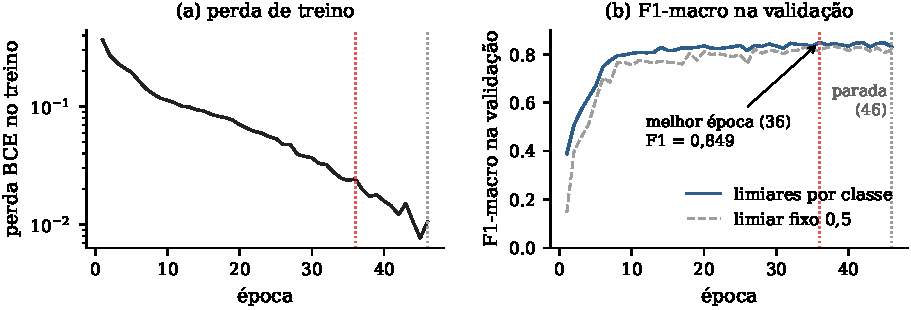
\includegraphics[width=0.66\textwidth]{figs/treino.pdf}
\caption{O F1 na validação estabiliza-se por volta da época 20, embora a perda no treino continue caindo, o que justificou a parada antecipada. (a) Perda no treino (escala logarítmica). (b) F1-macro na validação, com os limiares por classe e com o limiar fixo de 0,5. As linhas pontilhadas marcam a melhor época (36) e a parada (46).}\label{fig:treino}
\end{figure*}

\begin{figure}[!t]\centering
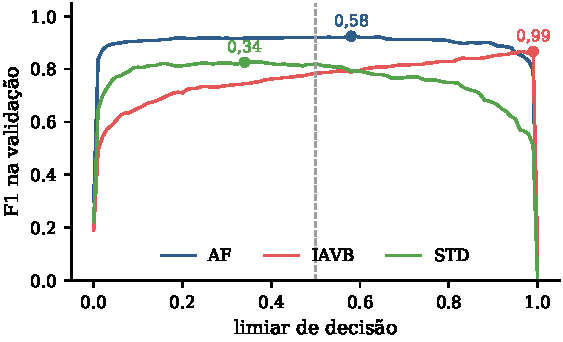
\includegraphics[width=\columnwidth]{figs/limiar.pdf}
\caption{O limiar de maior F1 é diferente em cada classe e, em várias delas, o F1 muda pouco numa faixa ampla de limiares. F1 na validação em função do limiar, para três classes; o ponto marca o limiar escolhido e a linha tracejada, o limiar de 0,5.}\label{fig:limiar}
\end{figure}

O modelo obteve F1-macro de 0,819 no teste, próximo do relatado por Zhang et al.\ na mesma base (0,813, média de 10 dobras)~\cite{zhang2021}. O F1 por classe também foi próximo do da referência (Tabela~\ref{tab:f1}): AF e BRD ficaram acima de 0,92, e STE foi a pior classe nos dois casos. Essa ordem das classes pelo F1 é a referência das comparações seguintes.

\begin{table*}[!t]\centering
\caption{O F1 por classe é próximo do relatado na referência, com AF e BRD no alto e STE em último. F1 por classe no teste, com os limiares por classe e com o limiar de 0,5; F1 de Zhang et al.~\cite{zhang2021} (média de 10 dobras); e número de mapas explicados (predições corretas). Classes ordenadas pelo F1 deste estudo.}\label{tab:f1}
\begin{tabular}{lrrrrrrrrr|r}
\toprule
& AF & BRD & IAVB & BRE & CVP & SNR & STD & CAP & STE & Macro \\
\midrule
F1 (limiares por classe) & 0,931 & 0,927 & 0,884 & 0,870 & 0,837 & 0,796 & 0,778 & 0,750 & 0,596 & 0,819 \\
F1 (limiar 0,5) & 0,931 & 0,921 & 0,811 & 0,857 & 0,814 & 0,772 & 0,778 & 0,750 & 0,622 & 0,806 \\
F1, Zhang et al.~\cite{zhang2021} & 0,919 & 0,926 & 0,864 & 0,866 & 0,851 & 0,805 & 0,814 & 0,735 & 0,535 & 0,813 \\
Mapas explicados & 108 & 172 & 61 & 20 & 59 & 78 & 65 & 45 & 14 & 622 \\
\bottomrule
\end{tabular}
\end{table*}

\subsection{Variação própria do GradientSHAP}
O piso médio foi de 0,18, de 0,13 em BRD e BRE a 0,25 em CAP (Tabela~\ref{tab:res}). Com 50 sorteios por mapa, ele era de 0,36.

\subsection{Métricas por classe}
A Tabela~\ref{tab:res} traz o valor de cada métrica por classe, e a Tabela~\ref{tab:ordens}, a ordem das classes em cada uma. Nenhuma métrica reproduziu exatamente a ordem do F1. As métricas se dividiram em dois grupos.

\begin{table*}[!t]\centering
\caption{As métricas de fidelidade e de robustez favorecem BRD e BRE, enquanto a \CS\ e o \RL\ acompanham o F1 nas pontas. Métricas por classe, com as classes na ordem do F1. FC: \FC\ ($|S| = 9$). FE: \FE. Max-S: \MS. N.º efet.: número efetivo de regiões (\CX). Cons.: \CS\ (entre parênteses, o valor ao acaso). RL: distância do \RL\ às classes ausentes. Setas: sentido melhor.}\label{tab:res}
\begin{tabular}{lrrrrrrrr}
\toprule
\textbf{Classe} & \textbf{F1} & \textbf{FC} $\uparrow$ & \textbf{FE} $\uparrow$ & \textbf{Max-S} $\downarrow$ & \textbf{Piso} & \textbf{N.º efet.} $\downarrow$ & \textbf{Cons.} $\uparrow$ & \textbf{RL} $\uparrow$ \\
\midrule
AF   & 0,931 & 0,544 & 0,515 & 0,056 & 0,19 & 22,9 & 0,457 (0,145) & 1,687 \\
BRD  & 0,927 & 0,746 & 0,784 & 0,029 & 0,13 & 22,2 & 0,723 (0,231) & 1,632 \\
IAVB & 0,884 & 0,647 & 0,553 & 0,041 & 0,18 & 23,0 & 0,424 (0,081) & 1,607 \\
BRE  & 0,870 & 0,651 & 0,698 & 0,033 & 0,13 & 26,2 & 0,335 (0,026) & 1,622 \\
CVP  & 0,837 & 0,618 & 0,659 & 0,047 & 0,17 & 25,0 & 0,382 (0,078) & 1,626 \\
SNR  & 0,796 & 0,448 & 0,493 & 0,049 & 0,23 & 26,2 & 0,260 (0,104) & 1,479 \\
STD  & 0,778 & 0,471 & 0,491 & 0,056 & 0,23 & 26,9 & 0,389 (0,086) & 1,483 \\
CAP  & 0,750 & 0,503 & 0,544 & 0,066 & 0,25 & 25,4 & 0,163 (0,059) & 1,578 \\
STE  & 0,596 & 0,633 & 0,592 & 0,045 & 0,18 & 25,5 & 0,084 (0,018) & 1,426 \\
\midrule
Global & 0,819 & 0,600 & 0,611 & 0,045 & 0,18 & 24,1 & 0,455 & 1,595 \\
\bottomrule
\end{tabular}
\end{table*}

\begin{table}[!t]\centering
\caption{Nenhuma métrica reproduz a ordem do F1; a \CS\ e o \RL\ coincidem com ele nas pontas. Ordem das classes em cada métrica, da melhor (1.ª) para a pior (9.ª).}\label{tab:ordens}
\setlength{\tabcolsep}{2.2pt}
\footnotesize
\begin{tabular}{lccccccccc}
\toprule
& 1.ª & 2.ª & 3.ª & 4.ª & 5.ª & 6.ª & 7.ª & 8.ª & 9.ª \\
\midrule
F1 & AF & BRD & IAVB & BRE & CVP & SNR & STD & CAP & STE \\
\midrule
Cons. & BRD & AF & IAVB & STD & CVP & BRE & SNR & CAP & STE \\
RL & AF & BRD & CVP & BRE & IAVB & CAP & STD & SNR & STE \\
FC & BRD & BRE & IAVB & STE & CVP & AF & CAP & STD & SNR \\
FE & BRD & BRE & CVP & STE & IAVB & CAP & AF & SNR & STD \\
Max-S & BRD & BRE & IAVB & STE & CVP & SNR & AF & STD & CAP \\
N.º efet. & BRD & AF & IAVB & CVP & CAP & STE & SNR & BRE & STD \\
\bottomrule
\end{tabular}
\end{table}

\paragraph{Métricas que acompanharam o F1 nas pontas} A \CS\ global foi de 0,455, acima do valor esperado ao acaso em todas as classes. As três classes de maior F1 (AF, BRD e IAVB) foram as três de maior \CS, e as duas de menor F1 (CAP e STE) foram as duas de menor \CS; com 1 e 3 regiões na discretização, essas pontas se mantiveram. No \RL, o mapa da classe explicada ficou, em média, a 1,60 do mapa de uma classe ausente no mesmo ECG, cerca de 10 vezes o piso do próprio mapa, e todos os 4\,886 pares ficaram acima do piso. AF teve as explicações mais específicas e STE, as menos; as cinco classes de maior F1 ocuparam as cinco primeiras posições.

\paragraph{Métricas que não acompanharam o F1} A \FC\ global foi de 0,60 e a \FE, de 0,61. BRD ficou no topo das duas, mas AF, a classe de maior F1, foi apenas a 6.ª na \FC\ e a 7.ª na \FE, e STE, a de menor F1, foi a 4.ª nas duas. As classes reconhecidas pela forma do QRS (BRD, BRE e CVP) ficaram no alto, e as de ritmo e onda P (SNR, AF e CAP) e a de depressão do segmento ST (STD) ficaram embaixo; com 4 e 18 regiões por subconjunto, BRD continuou em primeiro e STD e SNR, nas duas últimas posições. A \MS\ global foi de 0,045 e a \AS, de 0,036, cerca de quatro vezes menores que o piso: uma perturbação pequena do ECG mudou a explicação menos do que repetir o GradientSHAP com outra semente. Com 50 sorteios em vez de 200, a \MS\ era de 0,072. A ordem das classes na sensibilidade repetiu a da fidelidade.

\paragraph{Complexidade} Os mapas usaram, em média, o equivalente a 24 das 36 regiões. BRD, AF e IAVB tiveram os mapas mais concentrados (22 a 23 regiões), coincidindo com as três classes de maior F1, mas BRE, 4.ª no F1, ficou entre as mais espalhadas, e CAP e STE ficaram no meio. Com 50 sorteios, o valor era praticamente o mesmo (24,2).

\paragraph{Dependência do modelo} Com os pesos da rede sorteados de novo, o mapa não ficou mais espalhado: o número efetivo de regiões passou de 24,1 para 22,9, e o aumento relativo da entropia foi $q = -0{,}015$, com apenas 37\% dos mapas com $q > 0$. No modelo aleatório, as duas regiões principais foram de QRS em 88\% dos mapas, contra 42\% no modelo treinado, em que essa fração variou entre as classes (95\% em BRE e 71\% em BRD, contra 2\% em IAVB e 6\% em STD). Ainda assim, a distância entre o mapa do modelo treinado e o do aleatório foi, em média, 8,7 vezes o piso, e a região principal coincidiu em apenas 5\% dos casos.

\subsection{Robustez à definição das regiões}
Nas 9 combinações de limites, a \CS\ global variou de 0,414 a 0,469 e o número efetivo de regiões, de 23,7 a 24,5 (Tabela~\ref{tab:robreg}). As pontas da ordem das classes se mantiveram em todas as combinações: na \CS, BRD foi a primeira e CAP e STE ocuparam as duas últimas posições; na \CX, BRD, AF e IAVB foram as três mais concentradas e STD, a mais espalhada. As métricas que exigem passar ECGs modificados pelo modelo não foram recalculadas com os limites alternativos.

\begin{table}[!t]\centering
\caption{Os valores globais variam pouco com os limites das regiões. \CS\ e número efetivo de regiões (\CX) nas 9 combinações de limites; em negrito, a definição usada.}\label{tab:robreg}
\begin{tabular}{ccccc}
\toprule
& & \multicolumn{3}{c}{\textbf{Fim do ST-T (fração do RR)}} \\
\textbf{Métrica} & \textbf{QRS} & 0,40 & 0,45 & 0,50 \\
\midrule
\multirow{3}{*}{\CS} & 140~ms & 0,458 & 0,469 & 0,467 \\
 & 180~ms & 0,441 & \textbf{0,455} & 0,453 \\
 & 220~ms & 0,414 & 0,427 & 0,441 \\
\midrule
\multirow{3}{*}{N.º efet.} & 140~ms & 24,1 & 24,3 & 24,5 \\
 & 180~ms & 23,8 & \textbf{24,1} & 24,3 \\
 & 220~ms & 23,7 & 24,0 & 24,2 \\
\bottomrule
\end{tabular}
\end{table}

\section{Discussão}\label{sec:discussao}

Os resultados indicam que a qualidade das explicações GradientSHAP não acompanha o desempenho do modelo de forma única: depende da propriedade medida. As métricas que envolvem a decisão do modelo entre classes acompanharam o F1 nas pontas, enquanto as de fidelidade e de robustez seguiram outro padrão, ligado ao tipo de evidência de cada classe.

\subsection{Fidelidade e robustez seguem a evidência, e não o F1}
Os valores de fidelidade são compatíveis com a literatura. Em quatro bases de ECG, a \FC\ do DeepSHAP, outra aproximação dos valores SHAP, ficou entre 0,41 e 0,63, a maior entre os onze métodos avaliados~\cite{suh2024}; e, na mesma base deste estudo, a relevância atribuída pelos métodos funcionou mais como uma ordem de importância do que como uma contribuição proporcional~\cite{turbe2023}, o que torna esperadas correlações moderadas como as obtidas (0,60 e 0,61).

A ordem das classes na fidelidade concorda com o viés de amplitude descrito para os métodos que multiplicam o gradiente pela entrada ou subtraem uma referência, que deslocam a relevância para os componentes de maior amplitude do ECG~\cite{gumpfer2026}. No mesmo trabalho, esses métodos, entre eles o GradientSHAP, reforçaram as regiões de grande amplitude e falharam em cobrir o segmento ST na isquemia~\cite{gumpfer2026}. No presente estudo, as classes reconhecidas pela forma do QRS, o componente de maior amplitude do traçado, ficaram no topo da fidelidade, e as classes cuja evidência é um desvio pequeno (STD, onda P na CAP) ou uma propriedade da sequência de batimentos (a irregularidade do ritmo na AF) ficaram embaixo. Em dados sintéticos com evidência conhecida, variações simples de amplitude ou de duração do padrão entre as classes bastaram para produzir efeitos dependentes da classe, e as métricas de perturbação e as baseadas na evidência conhecida frequentemente avaliaram as classes de forma contraditória~\cite{baer2025b}. A diferença de fidelidade entre as classes não deve, portanto, ser lida por si como diferença de qualidade das explicações; Baer et al.\ mostram que a eficácia das perturbações varia muito entre as classes e recomendam complementar as médias agregadas com análises estratificadas por classe~\cite{baer2025a}. A AF ilustra o caso: retirar uma região não retira a irregularidade dos intervalos RR, e a queda da saída deixa de acompanhar a atribuição.

Na robustez, a principal fonte de variação das explicações foi o próprio método. As sensibilidades ficaram cerca de quatro vezes abaixo do piso, e a \MS\ caiu de 0,072 para 0,045 ao passar de 50 para 200 sorteios, o que mostra que parte da sensibilidade medida com poucos sorteios era erro de estimativa. Esse comportamento é coerente com a comparação de Mercier et al., em séries temporais, em que os métodos baseados em SHAP estiveram entre os de maior sensibilidade e os métodos de gradiente foram descritos como ruidosos e fracos nesse critério~\cite{mercier2022}, e mostra por que a leitura em relação ao piso é necessária: sem ela, a variação do método seria interpretada como falta de robustez da explicação. As classes menos robustas (CAP, STD e AF) foram também as de piso mais alto, isto é, aquelas em que o próprio método é menos estável, de novo as classes cuja evidência é pequena ou distribuída no tempo.

\subsection{Consistência e especificidade acompanham o F1}
A \CS\ foi a métrica cuja ordem mais se aproximou da ordem do F1. Duas propriedades da métrica contribuem para isso. Ela usa as predições do próprio modelo~\cite{dasgupta2022}, de modo que uma classe reconhecida por um padrão estável tende a produzir explicações repetidas e, ao mesmo tempo, um F1 alto. E ela depende do número de mapas de cada classe: BRD, com 172 mapas, teve o maior valor ao acaso (0,23), e STE, com 14, um valor ao acaso de 0,02, o que exige ler cada classe junto com o seu valor ao acaso.

No \RL, todos os pares ficaram acima do piso, de modo que os mapas não são o mesmo mapa para qualquer classe, falha que motivou a proposta da métrica~\cite{sixt2020}. Em EEG simulado, métodos da família gradiente × entrada também foram sensíveis à classe e à randomização do modelo~\cite{ravindran2023}. O fato de STE, a classe de menor F1, ter as explicações menos específicas é coerente com um modelo que separa pior essa classe das demais: se a evidência usada para STE se parece com a usada para outras classes, os mapas também se parecem.

\subsection{Complexidade e dependência do modelo}
A relação da complexidade com o F1 foi apenas parcial, e a complexidade foi a categoria de métricas menos confiável numa meta-avaliação das métricas~\cite{hedstrom2023metaquantus}, que recomenda não estimar a qualidade das explicações por uma única categoria. Por isso, ela foi lida em conjunto com as demais.

O \EM\ não foi satisfeito: o mapa do modelo aleatório ficou mais concentrado, e não mais espalhado. Isso é esperado num método que multiplica o gradiente por (ECG $-$ referência), Eq.~\eqref{eq:gshap}: sem o que o modelo aprendeu, o segundo fator continua presente e é maior nos picos do QRS, de modo que o mapa reproduz a forma do próprio ECG. Para métodos do tipo gradiente × entrada, a randomização dos pesos altera o sinal das atribuições, mas a estrutura da entrada permanece nos mapas~\cite{adebayo2018}; no ECG, o mesmo viés coloca a relevância no pico R mesmo em tarefas sobre as ondas P e T~\cite{wagner2024}. A entropia não capta essa diferença, mas as distâncias captam: o mapa do modelo aleatório ficou a 8,7 vezes o piso do mapa treinado, o que concorda com a perda rápida de correlação entre os mapas à medida que os pesos são randomizados, observada em ResNets para ECG~\cite{arends2026}. O mapa depende, portanto, do modelo, e o \EM\ foi tomado como teste de sanidade, e não como métrica de comparação entre classes.

\subsection{Resposta à pergunta do estudo}
Os resultados respondem à pergunta de forma condicional. A qualidade das explicações acompanha o desempenho do modelo nas propriedades que dependem da forma como o modelo separa as classes, a consistência entre explicação e predição e a especificidade da explicação para a classe, a mesma capacidade que o F1 mede. Ela não acompanha o desempenho na fidelidade e na robustez, que dependem da amplitude e da extensão da evidência de cada classe e, no GradientSHAP, do viés do método para os componentes de grande amplitude do ECG. Para o uso clínico das explicações, isso significa que o F1 de uma classe não indica, sozinho, se as suas explicações são fiéis ao modelo.

\subsection{Limitações}
Retirar regiões cria ECGs diferentes dos vistos no treino, e a queda da saída pode refletir, em parte, essa diferença e não apenas a perda de informação~\cite{ismail2020}. Perturbar trechos contíguos introduz menos ruído de alta frequência que perturbar pontos espalhados~\cite{cui2023}, e as duas referências testadas deram o mesmo resultado, mas o efeito não foi eliminado. Foi avaliado um único modelo treinado, e mapas de modelos treinados com sementes diferentes concordam apenas moderadamente~\cite{arends2026}; o piso mede a variação do método, e não a do treino. BRE (20 mapas) e STE (14) têm posições menos estáveis. O CPSC2018 não anota as regiões diagnósticas, de modo que a plausibilidade clínica das explicações não foi avaliada, e ela pode discordar da fidelidade~\cite{storas2025}. Os limites das regiões são aproximados, e o teste de robustez cobriu apenas a \CS\ e a \CX. A soma entre batimentos apaga variações de um batimento para outro, como a irregularidade do RR na AF ou um batimento prematuro isolado na CAP e na CVP. Por fim, o ruído do GradientSHAP não foi ajustado para o ECG.

\section{Conclusão}\label{sec:conclusao}

A qualidade das explicações GradientSHAP de redes neurais convolucionais para classificação de arritmias em ECG de 12 derivações acompanha o desempenho do modelo por classe apenas nas propriedades que dependem da decisão do modelo entre as classes. Explicações de classes reconhecidas com F1 mais alto são mais consistentes e mais específicas da classe, enquanto a fidelidade e a robustez refletem a amplitude e o tipo da evidência de cada classe, favorecendo as classes definidas pela forma do QRS e desfavorecendo as de ritmo e de segmento ST, independentemente do F1.

O objetivo de verificar se a qualidade das explicações acompanha o desempenho foi, assim, alcançado com uma resposta que depende da propriedade medida. Um F1 alto numa classe não garante explicações mais fiéis, e diferenças de fidelidade entre classes não indicam, por si, diferenças de confiabilidade. A avaliação das explicações em ECG precisa, por isso, ser feita por classe, com métricas de mais de uma categoria, calculadas sobre regiões fisiológicas do batimento e lidas em relação à variação do próprio método de explicação.


\bibliographystyle{IEEEtran}
\bibliography{referencias}

\end{document}
